%% Bookheader, Nov 8, 2020; July 18, 2022

\documentclass[11pt]{../Support/ourbook}
%% or for landscape, comment out line above and use this one:
%%\documentclass[landscape,11pt]{ourbook}

%% This will keep space from stretching around display math:

\makeatletter
\renewcommand\normalsize{%
   \@setfontsize\normalsize\@xipt{13.6}%
   \abovedisplayskip 11\p@  \@minus6\p@
   \abovedisplayshortskip \z@ 
   \belowdisplayshortskip 6.5\p@ \@minus3\p@
   \belowdisplayskip \abovedisplayskip
   \let\@listi\@listI}
\makeatother
\normalsize


\begin{document}

\tableofcontents
\graphicspath{{../../Chapters/polynomials_intro/en_US}}
\chapter{Introduction to Polynomials}

Watch Khan Academy's \textbf{Polynomials intro} video at \url{https://youtu.be/Vm7H0VTlIco}\index{polynomial}

A \emph{monomial}\index{monomial} is the product of a number and a variable raised to a non-negative (but possibly zero) integer power. Here are some examples of monomials:
\begin{multicols}{4}
  \begin{equation*}
    3 x^2
  \end{equation*}

  \begin{equation*}
    -2 x^{15}
  \end{equation*}

  \begin{equation*}
    \pi x^2
  \end{equation*}

  \begin{equation*}
    (3.33)x^{100}
  \end{equation*}

  \begin{equation*}
    7x
  \end{equation*}

  \begin{equation*}
    3
  \end{equation*}

  \begin{equation*}
    -\frac{2}{3}x^{12}
  \end{equation*}

  \begin{equation*}
    0
  \end{equation*}

  
\end{multicols}

The exponent is called the \emph{degree} of the monomial\index{monomial!degree}. For example, $3x^{17}$
has degree 17, $-7x$ has degree 1, and $3.2$ has degree 0 (because you can think of it as $(3.2)x^0$).\index{degree!polynomial}

The number in the product is called the \emph{coefficient}\index{monomial!coefficient}.  Example: $3x^{17}$ has a coefficient of 3, $-2x$ has a coefficient of -2, and $(3.4)x^{1000}$ has a coefficient of 3.4.\index{coefficient!polynomial}

A \emph{polynomial} \index{polynomial!definition of} is the sum of one or more monomials.  Here are some polynomials:
\begin{multicols}{3}
  \begin{equation*}
    4 x^2 + 9x + 3.9
  \end{equation*}

  \begin{equation*}
    -2 x^{10} + (3.4)x - 45x^{900} - 1
  \end{equation*}

  \begin{equation*}
    \pi x^2 + \pi x + \pi
  \end{equation*}

  \begin{equation*}
    3.3
  \end{equation*}

  \begin{equation*}
   7x + 2
  \end{equation*}

  \begin{equation*}
    3x^{20}
  \end{equation*}
\end{multicols}
We say that each monomial is a \emph{term} of the polynomial.

$x^{-5} + 12$ is \emph{not} a polynomial because the first term has a negative exponent.

$x^{2} - 32x^{\frac{1}{2}} + x$ is \emph{not} a polynomial because the second term has a non-integer exponent.

$\frac{x + 2}{x^2 + x + 5}$ is \emph{not} a polynomial because it is not just a sum of monomials.

\begin{Exercise}[title={Identifying Polynomials}, label=findpolynomials]
    Circle only the polynomials.
\begin{multicols}{3}
  \begin{equation*}
    -2 x^3 + \frac{1}{2}x + 3.9
  \end{equation*}

  \begin{equation*}
    2 x^{-10} + 4x - 1
  \end{equation*}
  
  \begin{equation*}
    (4.5)x^2 + \pi x
  \end{equation*}
  
  \begin{equation*}
    x^{\frac{2}{3}}
  \end{equation*}
  
  \begin{equation*}
   7
  \end{equation*}

  \begin{equation*}
    3x^{20} + 2x^{19} -5 x^{18}
  \end{equation*}
\end{multicols}
\end{Exercise}

\begin{Answer}[ref=findpolynomials]
\begin{multicols}{3}
  \begin{equation*}
    \boxed{-2 x^3 + \frac{1}{2}x + 3.9}
  \end{equation*}

  \begin{equation*}
    2 x^{-10} + 4x - 1
  \end{equation*}

  \begin{equation*}
    \boxed{(4.5)x^2 + \pi x}
  \end{equation*}

  \begin{equation*}
    x^{\frac{2}{3}}
  \end{equation*}

  \begin{equation*}
   \boxed{7}
  \end{equation*}

  \begin{equation*}
    \boxed{3x^{20} + 2x^{19} -5 x^{18}}
  \end{equation*}
\end{multicols}

\end{Answer}

We typically write a polynomial starting at the term with the highest
degree and proceed in decreasing order to the term with the lowest
degree:
\begin{equation*}
2 x^9 - 3x^7 + \frac{3}{4}x^3 + x^2 + \pi x -9.3
\end{equation*}
This is known as \emph{the standard form}.  The first term of the
standard form is called \emph{the leading term}, and we often call the
coefficient of the leading term \emph{the leading coefficient}.  We
sometimes speak of the degree of the polynomial, which is just the
degree of the leading term.\index{standard form!polynomial}

\begin{Exercise}[title={Standard of a Polynomial}, label=polynomialstandardform]
  Write $21x^2 - x^3 + \pi - 1000x$ in standard form. What is the degree of this polynomial? What is its leading coefficient?
\end{Exercise}
\begin{Answer}[ref=polynomialstandardform]
  Standard form would be $-x^3 + 21x^2 - 1000x + \pi$. The degree is 3. The leading coefficient is $-1$
\end{Answer}

\begin{Exercise}[title={Evaluate a Polynomial}, label=evaluatepolynomial]
  Let $y = x^3 - 3x^2 + 10x - 12$. What is $y$ when $x$ is $4$?
\end{Exercise}
\begin{Answer}[ref=evaluatepolynomial]
  $4^3 - (3)(4^2) + (10)(4) - 12 = 64 - 48 + 40 - 12$. So $y = 44$ 
\end{Answer}

We wouild be remiss in our duties if we didn't mention one more thing
about polynomials: Mathematicians have defined a polynomial to be a sum
of a \emph{finite} number of monomials.

It is certainly possible to have a sum of an infinite number of monomials
like this:
\begin{equation*}
1 + \frac{1}{2}x + \frac{1}{4}x^2 + \frac{1}{8}x^3 + \frac{1}{16}x^4 + \ldots
\end{equation*}
This is an example of an \emph{infinite series}, which we don't consider
polynomials. Infinite series are interesting and useful, but we 
will not discuss them in detail until later in the course.

\graphicspath{{../../Chapters/pylists/en_US}}
\chapter{Python Lists}

Watch CS Dojo's \textbf{Introduction to Lists in Python} video at \url{https://www.youtube.com/watch?v=tw7ror9x32s}

To review, Python list is an indexed collection. The indices start at
zero. You can create a list using square brackets.

You are now going to write a program that makes an array of
strings. Type this code into a file called \filename{faves.py}:

\begin{Verbatim}
favorites = ["Raindrops", "Whiskers", "Kettles", "Mittens"]
favorites.append("Packages")
print("Here are all my favorites:", favorites)
print("My most favorite thing is", favorites[0])
print("My second most favorite is", favorites[1])
number_of_faves = len(favorites)
print("Number of things I like:", number_of_faves)

for i in range(number_of_faves):
    print(i, ": I like", favorites[i])
\end{Verbatim}

Run it:
\begin{Verbatim}[commandchars=\\\{\}]
$ \textbf{python3 faves.py}
Here are all my favorites: ['Raindrops', 'Whiskers', 'Kettles', 'Mittens', 'Packages']
My most favorite thing is Raindrops
My second most favorite is Whiskers
Number of things I like: 5
0 : I like Raindrops
1 : I like Whiskers
2 : I like Kettles
3 : I like Mittens
4 : I like Packages
\end{Verbatim}
After you have run the code, study it until the output makes sense.

\begin{Exercise}[title={Assign into list}, label=assignintolist]
  Before you list the items, replace "Mittens" with "Gloves".
\end{Exercise}
\begin{Answer}[ref=assignintolist]
\begin{Verbatim}
favorites[3] = "Gloves"
\end{Verbatim}
\end{Answer}

\section{Evaluating Polynomials in Python}

First, before you go any further, you need to know that raising a
number to a power is done with ** in Python.  For example, to get
$5^2$, you would write \texttt{5**2}.

Back to polynomials: if you had a polynomial like $2x^3 -9x + 12$, you
could write it like this: $12x^0 + (-9)x^1 + 0x^2 + 2x^3$.  We could
use this representation to keep a polynomial in a Python list. We
would simply store all the coefficients in order:
\begin{Verbatim}
pn1 = [12,-9,0,2]
\end{Verbatim}

In the list, the index of each coefficient would correspond to the
degree of that monomial. For example, in the list, 2 is at index 3, so
that entry represents $2x^3$.

In the last chapter, you evaluated the polynomial $x^3 - 3x^2 + 10x -
12$ at $x=4$. Now you will write code that does that evalution.
Create a file called \filename{polynomials.py} and type in the following:

\begin{Verbatim}
def evaluate_polynomial(pn, x):
    sum = 0.0  
    for degree in range(len(pn)):
        coefficient = pn[degree]
        term_value = coefficient * x ** degree
        sum = sum + term_value
    return sum
   
pn1 = [-12.0, 10.0, -3.0, 1.0]
y = evaluate_polynomial(pn1, 4.0)
print("Polynomial 1: When x is 4.0, y is", y)
\end{Verbatim}

Run it. It should evaluate to 44.0.

\section{Walking the list backwards}

Now you are going to make a function that makes a pretty string to
represent your polynomial. Here is how it will be used:
\begin{Verbatim}
def polynomial_to_string(pn):
    ...Your Code Here...

pn_test = [-12.0, 10.0, 0.0, 1.0]
print(polynomial_to_string(pn1))
\end{Verbatim}

This would output:
\begin{Verbatim}
1.0x**3 + 10.0x + -12.0
\end{Verbatim}
This is not as simple as you might hope. In particular:
\begin{itemize}
\item You should skip the terms with a coefficient of zero
\item The term of degree 1 has an $x$, but no exponent
\item The term of degree 0 has neither an $x$ nor an exponent
\item Standard form demands that you list the terms in the reverse
  order from that of your coefficients list. You will need to walk the
  list from last to first.
\end{itemize}

Add this function to your \filename{polynomials.py} file after your \pyfunction{evaluate\_polynomial} function:
\begin{Verbatim}
  def polynomial_to_string(pn):
    
    # Make a list of the monomial strings
    monomial_strings = []

    # Start at the term with the largest degree
    degree = len(pn) - 1

    # Go through the list backwards stop after constant term
    while degree >= 0:
        coefficient = pn[degree]

        # Skip any term with a zero coefficient
        if coefficient != 0.0:

            # Describe the monomial
            if degree == 0:
                monomial_string = "{}".format(coefficient)
            elif degree == 1:
                monomial_string = "{}x".format(coefficient)
            else:
                monomial_string = "{}x^{}".format(coefficient, degree)
                
            # Add it to the list
            monomial_strings.append(monomial_string)

        # Move to the previous term
        degree = degree - 1

    # Deal with the zero polynomial
    if len(monomial_strings) == 0:
        monomial_strings.append("0.0")
    
    # Make a string that joins the terms with a plus sign
    return " + ".join(monomial_strings)
\end{Verbatim}

Note that in a list $n$ items, the indices go from 0 to $n-1$. When
we are walking the list backwards, we start at \pyfunction{len(pn) -
  1} and stop at zero.

Look over the code and google the functions you aren't familar
with. For example, if you want to know about the \pyfunction(join)
function, google for ``python join''.

Now, change your code to use the new function:
\begin{Verbatim}[commandchars=\\\{\}]
pn1 = [-12.0, 10.0, -3.0, 1.0]
y = evaluate_polynomial(pn1, 4.0)
\textbf{print("y =", polynomial\_to\_string(pn1))}
print("    When x is 4.0, y is", y)
\end{Verbatim}

Run the program. Does the function work?

\begin{Exercise}[title={Evaluate Polynomials}, label=pyevalpolynomials]
Using the function that you just wrote, add a few lines of code to
\filename{polynomials.py} to evaluate the following polynomials:
\begin{itemize}
\item Find $4x^4 - 7x^3 - 2x^2 + 5x + 2.5$ at $x = 8.5$.  It should be 16481.875
\item Find $5x^5 - 9$ at $x = 2.0$.  It should be 151.0
\end{itemize}
\end{Exercise}
\begin{Answer}[ref=pyevalpolynomials]
\begin{Verbatim}
pn2 = [2.5, 5.0, -2.0, -7.0, 4.0]
y = evaluate_polynomial(pn2, 8.5)
print("Polynomia 2: When x is 8.5, y is", y)

pn3 = [-9.0, 0.0, 0.0, 0.0, 0.0, 5.0]
y = evaluate_polynomial(pn3, 2.0)
print("Polynomial 3: When x is 2.0, y is", y)    
\end{Verbatim} 
\end{Answer}

\section{Plot the polynomial}

We can evaluate a polynomial at many points and plot them on a
graph. You are going to write the code to do this.  Create a new file
called \filename{plot\_polynomial.py}. Copy your \pyfunction{evaluate\_polynomial}
function into the new file.

Add a line at the beginning of the program that imports the plotting library matplotlib:
\begin{Verbatim}
import matplotlib.pyplot as plt
\end{Verbatim}

After the \pyfunction{evaluate\_polynomial} function:
\begin{itemize}
\item Create a list with polynomial coefficients.
\item Create two empty arrays, one for x values and one for y values.
\item Fill the x array with values from -3.5 to 3.5. Evaluate the polynomial at each of these points; put those values
  in the y array.
\item Plot them
\end{itemize}

Like this:
\begin{Verbatim}
# x**3 - 7x + 6
pn = [6.0, -7.0, 0.0, 1.0]

# These lists will hold our x and y values
x_list = []
y_list = []

# Start at x=-3.5
current_x =-3.5

# End at x=3.5
while current_x <= 3.5:
    current_y = evaluate_polynomial(pn, current_x)

    # Add x and y to respective lists
    x_list.append(current_x)
    y_list.append(current_y)

    # Move x forward
    current_x += 0.1

# Plot the curve
plt.plot(x_list, y_list)
plt.grid(True)
plt.show()
\end{Verbatim}

You should get a beautiful plot like this:

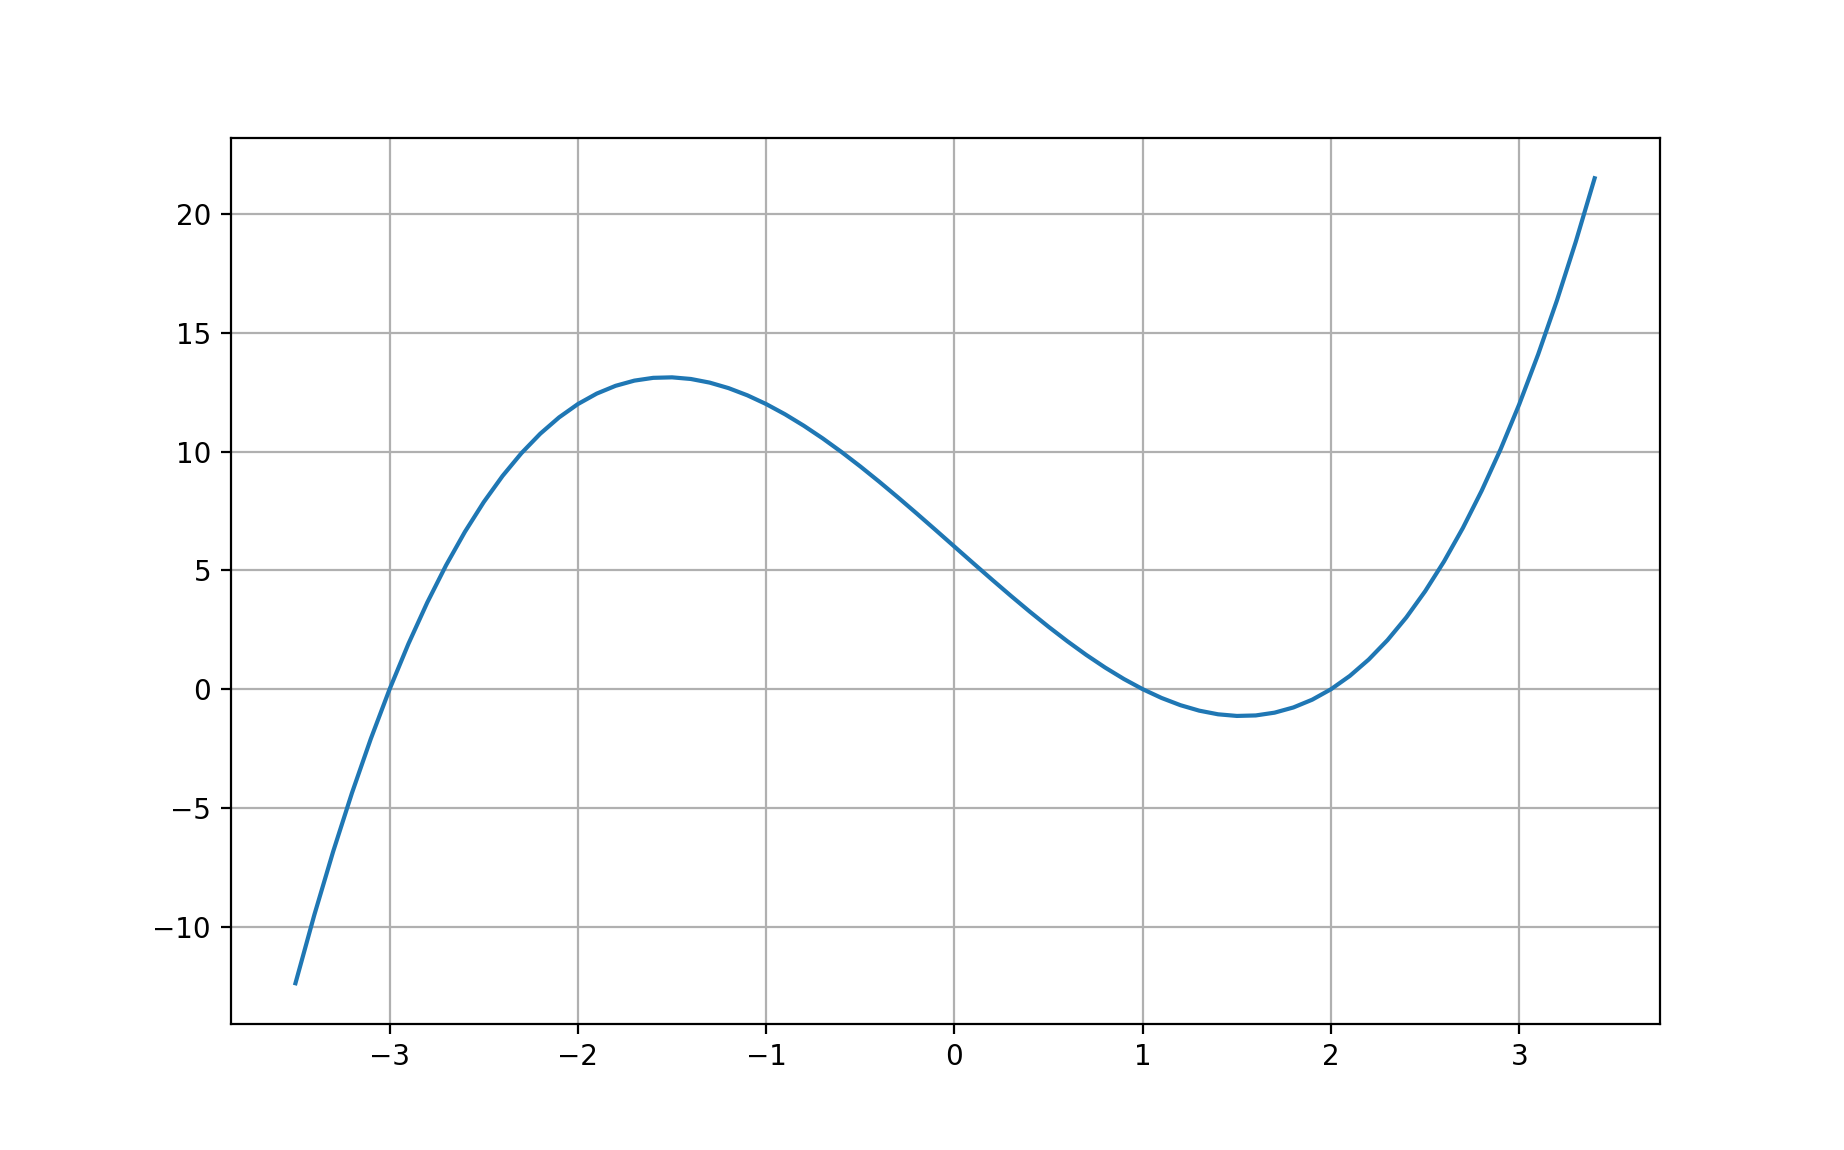
\includegraphics[width=\textwidth]{polyplot1.png}

If you received an error that the matplotlib was not found, use pip to install it:
\begin{Verbatim}[commandchars=\\\{\}]
$ \textbf{pip3 install matplotlib}
\end{Verbatim}

\begin{Exercise}[title={Observations}, label=plotobservations]
  Where does your polynomial cross the y-axis? Looking at the
  polynomial $x^3 - 7x + 6$, could you have guessed that value?

  \vspace{20mm}
  
  Where does your polynomial cross the x-axis? The places where a
  polynomial crosses the x-axis is called \emph{its roots}. Later in
  the course, you will learn techniques for finding the roots of a
  polynomial.
\end{Exercise}
\begin{Answer}[ref=plotobservations]
  The polynomial crosses the y-axis at 6. When x is zero, all the terms are zero except the
  last one. Thus, you can easily tell that $x^3 - 7x + 6$ will cross the y-axis at $y=6$.

  Looking at the graph, you tell that the curve crosses the y-axes
  near -3, 1 and 2. If you plug those numbers into the polynomial, you
  would find that it evalutes to zero at each one. Thus, $x=-3$, $x=1$, and $x=2$ are roots.
\end{Answer}

\graphicspath{{../../Chapters/add_subtract_polynomials/en_US}}
\chapter{Adding and Subtracting Polynomials}

Watch Khan Academy's \textbf{Adding polynomias} video at \url{https://youtu.be/ahdKdxsTj8E}

When adding two monomials of the same degree, you sum their coefficients:
\begin{equation*}
  7x^3 + 4x^3 = 11x^3
\end{equation*}\index{adding!monomials}

Using this idea, when adding two polynomials, you convert it into one long
polynomial and then simplify by combining terms with the same degree. For example:
\begin{multline*}
  (10x^3 - 2x + 13) + (-5x^2 + 7x -12) \\
  = 10x^3 + (-2)x + 13 + (-5)x^2 + 7x + (-12) \\
  = 10x^3 + (-5)x^2 + (-2 + 7)x + (13 - 12) \\
  = 10x^3 - 5x^2 + 5x + 1
\end{multline*}\index{adding!polynomials}

\begin{Exercise}[title=Adding Polynomials Practice, label=addpns]
  Add the following polynomials:
  \Question{$2x^3 - 5x^2 + 3x - 9$ and $x^3 - 2x^2 - 2x - 9$}
  \vspace{20mm}
  \Question{$3x^5 - 5x^3 + 3x^2 - x - 3$ and $2x^4 - 2x^3 - 2x^2 + x - 9$}
  \vspace{20mm}
\end{Exercise}
\begin{Answer}[ref=addpns]$3x^3 - 7x^2 + x - 18$ and $3x^5 - 7x^3 + x^2 - 12$\end{Answer}

Notice that in the second question, the degree 1 term disappears completely: $(-x) + x = 0$

One more tricky thing that can happen: Sometimes the coefficients don't add nicely.  For example:
\begin{equation*}
  \pi x^2 - 3 x^2 = (\pi - 3) x^2
\end{equation*}
That is as far as you can simplify it.
    
\section{Subtraction}

Now watch Khan Academy's \textbf{Subtracting polynomials} at \url{https://youtu.be/5ZdxnFspyP8}.

When subtracting one polynomial from the other, it is a lot like
adding two polynomials. The difference: when make the two polynomials
into one long polynomial, we multiply each monomial that is being
subtracted by -1. For example:
\begin{multline*}
  (2x^2 - 3x + 9) - (5x^2 - 7x + 4) \\
  = 2x^2 + (-3)x + 9 + (-5)x^2 + 7x + (-4) \\
  = (2 - 5)x^2 + (-3 + 7)x + (9-4) \\
  = -3x^2 + 4x + 5
\end{multline*}

\begin{Exercise}[title=Subtracting Polynomials Practice, label=subtractpns]
  Add the following polynomials:
  \Question{$(2x^3 - 5x^2 + 3x - 9) - (x^3 - 2x^2 - 2x - 9)$}
  \vspace{20mm}
  \Question{$(3x^5 - 5x^3 + 3x^2 - x - 3) - (2x^4 - 2x^3 - 2x^2 + x - 9)$}
  \vspace{20mm}
\end{Exercise}
\begin{Answer}[ref=subtractpns]$x^3 - 3x^2 + 5x$ and $x^5 - 3x^3 + 5x^2 - 2x + 6$\end{Answer}

\section{Adding Polynomials in Python}

As a reminder, in our Python code, we are representing a polynomial
with a list of coefficients.  The first coefficient is the constant
term. The last coefficient is the leading coefficient. So, we can
imagine $-5x^3 + 3x^2 - 4x + 9$ and $2x^3 +4x^2 - 9$ would look
like this: \textit{FIXME: Diagram here}

To add the two polynomials then, we sum the coefficients for each degree.
\textit{FIXME: Diagram here}

Create a file called \filename{add\_polynomials.py}, and type in the following: 
\begin{Verbatim}
def add_polynomials(a, b):
    degree_of_result = len(a)
    result = []
    for i in range(degree_of_result):
        coefficient_a = a[i]
        coefficient_b = b[i]
        result.append(coefficient_a + coefficient_b)
    return result

polynomial1 = [9.0, -4.0, 3.0, -5.0]
polynomial2 = [-9.0, 0.0, 4.0, 2.0]
polynomial3 = add_polynomials(polynomial1, polynomial2)

print('Sum =', polynomial3)
\end{Verbatim}

Run the program.

Unfortunately, this code only works if the polynomails are the same length. For
example, try making \pyvar{polynomial1} have a larger degree than
\pyvar{polynomial2}:
\begin{Verbatim}
# x**4 - 5x**3 + 3x**2 - 4x + 9
polynomial1 = [9.0, -4.0, 3.0, -5.0, 1.0]
  
# 2x**3 + 4x**2 - 9  
polynomial2 = [-9.0, 0.0, 4.0, 2.0]
polynomial3 = add_polynomials(polynomial1, polynomial2)
print('Sum =', polynomial3)
\end{Verbatim}

See the problem?

\begin{Exercise}[title=Dealing with polynomials of different degrees, label=pyaddpolys]
  
Can you fix the function \pyfunction{add\_polynomials} to handle polynomials of different degrees?

Here is a hint: In Python, there is a \pyfunction{max} function that returns the largest of the numbers it is passed.
\begin{Verbatim}
biggest = max(5,7)
\end{Verbatim}
Here \pyvar{biggest} would be set to 7.

Here is another hint: If you have an array \pyvar{mylist}, \pyvar{i},
a non-negative integer, is only a legit index if \texttt{i <
  len(mylist)}.
\end{Exercise}
\begin{Answer}[ref=pyaddpolys]
\begin{Verbatim}
def add_polynomials(a, b):
    degree_of_result = max(len(a), len(b))
    result = []
    for i in range(degree_of_result):
        if i < len(a):
            coefficient_a = a[i]
        else:
            coefficient_a = 0.0   

        if i < len(b):
            coefficient_b = b[i]
        else:
            coefficient_b = 0.0
            
        result.append(coefficient_a + coefficient_b)
    return result
\end{Verbatim}
\end{Answer}

\section{Scalar multiplication of  polynomials}

If you multiply a polynomial with a number, the distributive property applies:
\begin{equation*}
  (3.1)(2x^2 + 3x + 1) = (6.2)x^2 + (9.3)x + 3.1
\end{equation*}
(When we are talking about things that are more complicated than a number, we use the word \emph{scalar} to mean ``Just a number''. So this is the product of a scalar and a polynomial.)

In \filename{add\_polynomials.py}, add a function to that multiplies a scalar and a polynomial:
\begin{Verbatim}
def scalar_polynomial_multiply(s, pn):
    result = []
    for coefficient in pn:
        result.append(s * coefficient)
    return result
\end{Verbatim}

Somewhere near the end of the program, test this function:
\begin{Verbatim}
polynomial4 = scalar_polynomial_multiply(5.0, polynomial1)
print('Scalar product =', polynomial_to_string(polynomial4))
\end{Verbatim}

\begin{Exercise}[title=Subtract polynomials in Python, label=pysubpoly]
Now implement a function that does subtraction using
\pyfunction{scalar\_polynomial\_multiply} and
\pyfunction{add\_polynomials}.

It should look like this:
\begin{Verbatim}
def subtract_polynomial(a, b):
    ...Your code here...

polynomial5 = [9.0, -4.0, 3.0, -5.0]
polynomial6 = [-9.0, 0.0, 4.0, 2.0, 1.0]
polynomial7 = subtract_polynomial(polynomial5, polynomial6)
print('Difference =', polynomial_to_string(polynomial7))
\end{Verbatim}
\end{Exercise}
\begin{Answer}[ref=pysubpoly]
\begin{Verbatim}
def subtract_polynomial(a, b):
    neg_b = scalar_polynomial_multiply(-1.0, b)
    return add_polynomials(a, neg_b)
\end{Verbatim}
\end{Answer}


    

\graphicspath{{../../Chapters/multiplying_polynomials/en_US}}
\chapter{Multiplying Polynomials}

Watch Khan Academy's \textbf{Multiplying monomials} at \url{https://youtu.be/Vm7H0VTlIco}.

To review, when you multiply two monomials, you take the product of
their coefficients and the sum of their degrees:
\begin{equation*}
  (2x^6)(5x^3) = (2)(5)(x^6)(x^3) = 10x^9
\end{equation*}
If you have a product of more than two monomials, multiply \emph{all}
the coefficients and sum \emph{all} the exponents:
\begin{equation*}
  (3x^2)(2x^3)(4x) = (3)(2)(4)(x^2)(x^3)(x^1) = 24x^6
\end{equation*}\index{multiplication!polynomials}

\begin{Exercise}[title={Multiplying monomials}, label=multmonomials]
Multiply these monomials
  \Question $(3x^2)(5x^3)$
\vspace{20mm}
  \Question $(2x)(4x^9)$
\vspace{20mm}
  \Question $(-5.5x^2)(2x^3)$
\vspace{20mm}
  \Question $(\pi)(-2x^5)$
\vspace{20mm}
  \Question $(2x)(3x^2)(5x^7)$
\vspace{20mm}
\end{Exercise}
\begin{Answer}[ref=multmonomials]
  $(3x^2)(5x^3) = 15x^5$
  
  $(2x)(4x^9) = 8x^{10}$
  
  $(-5.5x^2)(2x^3) = -11x^5$

  $(\pi)(-2x^5) = -2\pi x^5$
  
  $(2x)(3x^2)(5x^7) = 30x^{10}$
\end{Answer}

\section{Multiplying a monomial and a polynomial}

Watch Khan Academy's \textbf{Multiplying monomials by polynomials} at \url{https://youtu.be/pD2-H15ucNE}.

When multiplying a monomial and a polynomial, you use the the distributive property. Then it is just multiplying several pairs of monomials:
\begin{multline*}
  (3x^2)(4x^3 - 2x^2 + 3x - 7) \\
  = (3x^2)(4x^3) + (3x^2)(-2x^2) + (3x^2)(3x) + (3x^2)(-7) \\
  = 12x^5 - 6x^4 + 9x^3 -21x^2
\end{multline*}

\begin{Exercise}[title={Multiplying a monomial and a polynomial}, label=multmonopoly]
Multiply these monomials
\Question $(3x^2)(5x^3 - 2x + 3)$
\vspace{20mm}
\Question $(2x)(4x^9 - 1)$
\vspace{20mm}
\Question $(-5.5x^2)(2x^3 + 4x^2 + 6)$
\vspace{20mm}
\Question $(\pi)(-2x^5 + 3x^4 + x)$
\vspace{20mm}
\Question $(2x)(3x^2)(5x^7 + 2x)$
\end{Exercise}
\begin{Answer}[ref=multmonopoly]
  $(3x^2)(5x^3 - 2x + 3) = 15x^6 - 6x^3 + 6x^2$

  $(2x)(4x^9 - 1) = 8x^{10} - 2x$

  $(-5.5x^2)(2x^3 + 4x^2 + 6) = 11x^5 - 22x^4 + 33x^2$

  $(\pi)(-2x^5 + 3x^4 + x) = -2\pi x^5 + 3\pi x^4 + \pi x$

  $(2x)(3x^2)(5x^7 + 2x) = 30x^{10} + 12x^4$
\end{Answer}

\section{Multiplying polynomials}

Watch Khan Academy's \textbf{Multiplying binomials by polynomials} video at \url{https://youtu.be/D6mivA_8L8U}

When you are multiplying two polynomials, you will use the
distributive property several times to make it one long
polynomial. Then you will combine the terms with the same degree. For
example,
\begin{multline*}
  (2x^2 - 3)(5x^2 + 2x - 7) \\
  =   (2x^2)(5x^2 + 2x - 7) + (-3)(5x^2 + 2x - 7) \\
  =   (2x^2)(5x^2) + (2x^2)(2x) + (2x^2)(-7) + (-3)(5x^2) + (-3)(2x) + (-3)(-7) \\
  =   10^4 + 4x^3 + -14x^2 + -15x^2 + -6x + 21
  =   10^4 + 4x^3 + -29x^2 + -6x + 21
\end{multline*}

One common form that you will see is multiplying two binomials together:
\begin{multline*}
(2x + 7)(5x + 3) = (2x)(5x + 3) + (7)(5x+3) = (2x)(5x) + (7)(5x) + (2x)(3) + (7)(3)
\end{multline*}
Notice the product has become the sum of four parts: the firsts, the
inners, the outers, and the lasts. People sometimes use the mnemonic
FOIL to remember this pattern, but there is a general rule that works
for all product of polynomials, not just binomials.  Here it is: Every
term in the first will be multiplied by every term in the second, and
then just add them together.

So, for example, if you have a polynomial $s$ with three terms and you
multiply it by a polynomial $t$ with five terms, you will get a sum of
15 terms -- each term is a product of two monomials, one from $s$ and
one from $t$.  (Of course, several of those terms might have the same
degree, so they will be combined together when you simplify. Thus you
typically end up with a polynomial with less than 15 terms.)

Using this rule, here is how I would multiply $2x^2 - 3x + 1$ and
$5x^2 + 2x - 7$:
\begin{multline*}
  (2x^2 - 3x + 1)(5x^2 + 2x - 7)  = \begin{matrix}
  (2x^2)(5x^2)& + &(2x^2)(2x)& + &(2x^2)(-7)& + \\
  (-3x)(5x^2)& + &(-3x)(2x)& + &(-3x)(-7)& + \\
    (1)(5x^2)& + &(1)(2x)& + &(1)(-7)& 
  \end{matrix} \\
  = 10x^4 + 4x^3 + (-14)x^2 + (-15)x^3 + (-6)x^2 + 21x +5x^2 + 2x + (-7) \\
  = 10x^4 + (4 - 15)x^3 + (-14 - 6 + 5)x^2  + (21 + 2)x + (-7) \\
  = 10x^4 - 11x^3 - 15x^2 + 23x - 7
\end{multline*}
Note that the product (before combining terms with the same degree) has
$3 \times 3 = 9$ terms -- every possible combination of a term from the
first polynomial and a term from the second polynomial.

One common source of error: losing track of the negative
signs. You will need to be really careful. I have found that it
helps to use + between all terms, and use negative coefficients to
express subtraction. For example, if the problem says $4x^2 - 5x - 3$,
you should work with that as $4x^2 + (-5)x + (-3)$

\begin{Exercise}[title={Multiplying polynomials}, label=multpolys]
  Multiply the following pairs of polynomials:
  \Question{$2x + 1$ and $3x - 2$}
  \vspace{15mm}
  \Question{$-3x^2 + 5$ and $4x -2$}
  \vspace{15mm}
  \Question{$-2x - 1$ and $-3x - \pi$}
  \vspace{15mm}
  \Question{$-2x^5 + 5x$ and $3x^5 + 2x$}
  \vspace{15mm}

\end{Exercise}
\begin{Answer}[ref=multpolys]
  $(2x + 1)(3x - 2) = 6x^2 - x - 2$

  $(-3x^2 + 5)(4x - 2) = -12x^3 + 6x^2 + 20x - 10$

  $(-2x - 1)(-3x - \pi) = 6x^2 + (4 + 2\pi)x + \pi$ 

  $(-2x^5 + 5x)(3x^5 + 2x) = -6x^{10} + 12x^6 + 10x^2$
\end{Answer}

\begin{Exercise}[title={Observations}, label=obsmultpoly]
  Let's say I have two polynomials, $p_1$ and $p_2$.  $p_1$ has degree
  23.  $p_2$ has degree 12.  What is the degree of their product?
\end{Exercise}
\begin{Answer}[ref=obsmultpoly]
  The degree of the product is determined by the term that is the
  product of the highest degree term in $p_1$ and the highest degree
  term in $p_2$. Thus, the product of a degree 23 polynomial and a
  degree 12 polynomial has degree 35.
\end{Answer}
  

\graphicspath{{../../Chapters/pymultpoly/en_US}}
\chapter{Multiplying Polynomials in Python}

At this point, you have created a nice toolbox of functions for
dealing with lists of coefficients as polynomials. Create a file called \filename{poly.py} and copy the folowing functions into it:
\begin{itemize}
\item \pyfunction{evaluate\_polynomial}
\item \pyfunction{polynomial\_to\_string}
\item \pyfunction{add\_polynomials}
\item \pyfunction{scalar\_polynomial\_multiply}
\item \pyfunction{subtract\_polynomial}
\end{itemize}

Now, create another file in the same directory called \filename{test.py}. Type this into that file:
\begin{Verbatim}
import poly

polynomial_a = [9.0, -4.0, 3.0, -5.0]
print('Polynomial A =', poly.polynomial_to_string(polynomial_a))

polynomial_b = [-9.0, 0.0, 4.0, 2.0, 1.0]
print('Polynomial B =', poly.polynomial_to_string(polynomial_b))

# Evaluation
value_of_b = poly.evaluate_polynomial(polynomial_b, 3)
print('Polynomial B at 3 =', value_of_b)

# Adding
a_plus_b = poly.add_polynomials(polynomial_a, polynomial_b)
print('A + B =', poly.polynomial_to_string(a_plus_b))

# Scalar multiplication
b_scalar = poly.scalar_polynomial_multiply(-3.2, polynomial_b)
print('-3.2 * Polynomial B =', poly.polynomial_to_string(b_scalar))

# Subtraction
a_minus_b = poly.subtract_polynomial(polynomial_a, polynomial_b)
print('A - B =', poly.polynomial_to_string(a_minus_b))
\end{Verbatim}

When you run it, you should get the following:
\begin{Verbatim}
Polynomial A = -5.0x^3 + 3.0x^2 + -4.0x + 9.0
Polynomial B = 1.0x^4 + 2.0x^3 + 4.0x^2 + -9.0
Polynomial B at 3 = 162.0
A + B = 1.0x^4 + -3.0x^3 + 7.0x^2 + -4.0x
-3.2 * Polynomial B = -3.2x^4 + -6.4x^3 + -12.8x^2 + 28.8
A - B = -1.0x^4 + -7.0x^3 + -1.0x^2 + -4.0x + 18.0
\end{Verbatim}

You are now ready to implement the multiplication of polynomials. The function will look like this:
\begin{Verbatim}
def multiply_polynomials(a, b):
  ...Your code here...
\end{Verbatim}
It will return a list of coefficients.

In an exercise in the last chapter, you were asked `` Let's say I have
two polynomials, $p_1$ and $p_2$.  $p_1$ has degree 23.  $p_2$ has
degree 12.  What is the degree of their product?'' The answer was $23 +
12 = 35$.

In our implementation, a polynomial of degree 23 is held in a list of length 24.

In Python, we wil be trying to multiply a polynomial $a$ and a
polynomial $b$ represented as lists. What is the degree of that product?
\begin{Verbatim}
      result_degree = (len(a) - 1) + (len(b) - 1)
\end{Verbatim}

Now, we need to create an array of zeros that is one longer than that. Here is a cute Python trick: If you have a list, you can replicate it using the * operator. 
\begin{Verbatim}
a = [5,7]
b = a * 4
print(b)
# [5, 7, 5, 7, 5, 7, 5, 7]
\end{Verbatim}

Here iss how you will get a list of zeros:
\begin{Verbatim}
      result = [0.0] * (result_degree + 1)
\end{Verbatim}

We will step through $a$, getting the index and value of each entry. You can do this in one line using \pyfunction{enumerate}:
\begin{Verbatim}
      for a_degree, a_coefficient in enumerate(a):
\end{Verbatim}
For each of those, we will step through the entire $b$ polynomial. As
you multiply together each term, you will add it to the appropriate
coefficient of the result.

Here is the whole function:
\begin{Verbatim}
def multiply_polynomials(a, b): # What is the degree of the resulting
polynomial?  result_degree = (len(a) - 1) + (len(b) - 1)

    # Make a list of zeros to hold the coefficents result = [0.0] *
    (result_degree + 1)

    # Iterate over the indices and values of a for a_degree,
    a_coefficient in enumerate(a):

        # Iterate over the indices and values of b for b_degree,
        b_coefficient in enumerate(b):

            # Calculate the resulting monomial coefficient =
            a_coefficient * b_coefficient degree = a_degree + b_degree
            
            # Add it to the right bucket
            result[degree] = result[degree] + coefficient
            
    return result
\end{Verbatim}

Take a long look at that function.  When you understand it, type it into \filename{poly.py}.

In \filename{test.py}, try out the new function:
\begin{Verbatim}
# Multiplication
a_times_b = poly.multiply_polynomials(polynomial_a, polynomial_b)
print('A x B =', poly.polynomial_to_string(a_times_b))
\end{Verbatim}

This is an example of a \emph{nested loop}. The outer loop steps
through the polynomial $a$. For each step it takes, the inner loop
steps through the entire polynomial $b$.

\section{Something surprising about lists}

You can imagine that you might want to create two very similar polynomials. Let's say polynomial $c$ is $x^2 + 2x + 1$ and polynomial $d$ is $x^2 -2x + 1$.  You might think you are very clever to just alter that degree 1 coefficient like this:
\begin{Verbatim}
c = [1.0, 2.0, 1.0]
d = c
d[1] = -2.0
\end{Verbatim}

If you printed out $c$, you would get $[1.0, -2.0, 1.0]$.  Why? You
assigned two variables ($c$ and $d$) to the \emph{the same list}.  So,
when you use one reference ($d$) to change the list, you see the
change if you look at the list from either reference. \emph{FIXME:
  Diagram of two references to the same list here.}

To create two separate lists, you would need to explicitly make a copy:
\begin{Verbatim}
c = [1.0, 2.0, 1.0]
d = c.copy()
d[1] = -2.0
\end{Verbatim}


%%%%%%%%%%%%%%%%%%%%%%%%%%%%%%%%%
%% Bookfooter.tex by Aaron Hillegass
%% Nov 8, 2020

\appendix

\chapter{Answers to Exercises}
\shipoutAnswer

\bibliography{references}

\printindex

\end{document}